
\documentclass[11pt,a4paper]{article}
\usepackage[T1]{fontenc}
\usepackage{lmodern}
\usepackage{amsmath,amssymb,amsfonts,mathtools}
\usepackage{graphicx,booktabs,longtable,array,tabularx,adjustbox}
\usepackage{geometry,microtype,fancyhdr,lastpage,etoolbox,enumitem}
\usepackage{newunicodechar,textcomp}
\usepackage{hyperref}
\hypersetup{hidelinks,pdfcreator={XeLaTeX / QM1 academic edition}}
\geometry{left=20mm,right=20mm,top=22mm,bottom=23mm}
\setcounter{secnumdepth}{2}
\setlength{\parindent}{0pt}
\setlength{\parskip}{4pt plus 1pt}
\setlength{\emergencystretch}{2em}
\setlength{\tabcolsep}{3pt}
\renewcommand{\arraystretch}{1.16}
\setlist{nosep,topsep=3pt,itemsep=2pt,leftmargin=7mm}
\AtBeginEnvironment{longtable}{\footnotesize\setlength{\tabcolsep}{2.2pt}}
\newcommand{\tightlist}{\setlength{\itemsep}{0pt}\setlength{\parskip}{0pt}}
\providecommand{\Cov}{\operatorname{Cov}}
\providecommand{\Var}{\operatorname{Var}}
\providecommand{\Corr}{\operatorname{Corr}}
\providecommand{\MAD}{\operatorname{MAD}}
\providecommand{\E}{\mathbb{E}}
\providecommand{\R}{\mathbb{R}}
\newunicodechar{—}{\textemdash}
\newunicodechar{–}{\textendash}
\newunicodechar{€}{\texteuro}
\newunicodechar{≤}{\ensuremath{\leq}}
\newunicodechar{≥}{\ensuremath{\geq}}
\newunicodechar{×}{\ensuremath{\times}}
\newunicodechar{÷}{\ensuremath{\div}}
\newunicodechar{Σ}{\ensuremath{\Sigma}}
\newunicodechar{σ}{\ensuremath{\sigma}}
\newunicodechar{μ}{\ensuremath{\mu}}
\newunicodechar{Δ}{\ensuremath{\Delta}}
\newunicodechar{∑}{\ensuremath{\sum}}
\newunicodechar{≈}{\ensuremath{\approx}}
\newunicodechar{√}{\ensuremath{\surd}}
\newunicodechar{≠}{\ensuremath{\ne}}
\newunicodechar{→}{\ensuremath{\to}}
\newunicodechar{∞}{\ensuremath{\infty}}
\newunicodechar{∈}{\ensuremath{\in}}
\newunicodechar{−}{\ensuremath{-}}
\newunicodechar{²}{\ensuremath{^{2}}}
\newunicodechar{³}{\ensuremath{^{3}}}
\newunicodechar{₀}{\ensuremath{_{0}}}
\newunicodechar{₁}{\ensuremath{_{1}}}
\newunicodechar{₂}{\ensuremath{_{2}}}
\newunicodechar{₃}{\ensuremath{_{3}}}
\newunicodechar{₄}{\ensuremath{_{4}}}
\newunicodechar{ₜ}{\ensuremath{_{t}}}
\newunicodechar{ₚ}{\ensuremath{_{p}}}
\newunicodechar{ₙ}{\ensuremath{_{n}}}
\newunicodechar{ₓ}{\ensuremath{_{x}}}
\newunicodechar{ᵢ}{\ensuremath{_{i}}}
\newunicodechar{ŷ}{\ensuremath{\hat y}}
\newunicodechar{Ŷ}{\ensuremath{\widehat Y}}
\newunicodechar{ₘ}{\ensuremath{_{m}}}
\newunicodechar{ₑ}{\ensuremath{_{e}}}
\newunicodechar{ₐ}{\ensuremath{_{a}}}
\newunicodechar{ₖ}{\ensuremath{_{k}}}
\newunicodechar{ₛ}{\ensuremath{_{s}}}
\newunicodechar{ₗ}{\ensuremath{_{l}}}
\newunicodechar{ₕ}{\ensuremath{_{h}}}
\newunicodechar{ₒ}{\ensuremath{_{o}}}
\newunicodechar{₊}{\ensuremath{_{+}}}
\newunicodechar{₋}{\ensuremath{_{-}}}
\newunicodechar{₌}{\ensuremath{_{=}}}
\newunicodechar{₍}{\ensuremath{_{(}}}
\newunicodechar{₎}{\ensuremath{_{)}}}
\newunicodechar{⁻}{\ensuremath{^{-}}}
\newunicodechar{⁺}{\ensuremath{^{+}}}
\newunicodechar{⁰}{\ensuremath{^{0}}}
\newunicodechar{¹}{\ensuremath{^{1}}}
\newunicodechar{⁴}{\ensuremath{^{4}}}
\newunicodechar{⁵}{\ensuremath{^{5}}}
\newunicodechar{⁶}{\ensuremath{^{6}}}
\newunicodechar{⁷}{\ensuremath{^{7}}}
\newunicodechar{⁸}{\ensuremath{^{8}}}
\newunicodechar{⁹}{\ensuremath{^{9}}}
\makeatletter
\renewcommand{\section}{\@startsection{section}{1}{0pt}{2.0ex plus .7ex minus .3ex}{1.0ex}{\large\bfseries}}
\renewcommand{\subsection}{\@startsection{subsection}{2}{0pt}{1.8ex plus .5ex minus .2ex}{.7ex}{\normalsize\bfseries}}
\renewcommand{\subsubsection}{\@startsection{subsubsection}{3}{0pt}{1.3ex plus .4ex minus .2ex}{.5ex}{\normalsize\bfseries}}
\makeatother
\pagestyle{fancy}
\fancyhf{}
\renewcommand{\headrulewidth}{0.35pt}
\renewcommand{\footrulewidth}{0pt}
\fancyhead[L]{\small\textsc{KEDGE Business School --- QM1}}
\fancyhead[R]{\small\textsc{2026--2027}}
\fancyfoot[L]{\small Badr ABOUFARASSE, PhD}
\fancyfoot[R]{\small\thepage\ /\ \pageref{LastPage}}
\setlength{\headheight}{14pt}
\setkeys{Gin}{keepaspectratio}
\begin{document}

\begin{center}
{\small\textsc{KEDGE Business School \quad EBP1 \quad Quantitative Methods 1}}\\[6pt]
{\Large\bfseries Fiche 1 — Présenter et organiser les données}\\[6pt]
{\normalsize\bfseries Corrigés intégralement détaillés}\\[6pt]
{\small Badr ABOUFARASSE, PhD \quad --- \quad 2026--2027}
\end{center}
\vspace{2mm}\hrule\vspace{6mm}

\hypertarget{applications-fondamentales}{%
\section{Applications fondamentales}\label{applications-fondamentales}}

Maîtriser les définitions et les calculs essentiels du cours.

\emph{Application du cours --- 10 min}

\hypertarget{exercice-1-population-uxe9chantillon-et-nature-des-variables}{%
\subsection{Exercice 1 -- Population, échantillon et nature des variables}\label{exercice-1-population-uxe9chantillon-et-nature-des-variables}}

Un magasin souhaite étudier l'ensemble de ses clients ayant effectué un achat au mois de septembre. Il interroge un échantillon de 80 clients et relève :

\begin{longtable}[]{@{}p{0.32\linewidth}p{0.62\linewidth}@{}}
\toprule\noalign{}
Variable & Exemple \\
\midrule\noalign{}
\endhead
\bottomrule\noalign{}
\endlastfoot
Mode de paiement & carte, espèces, mobile \\
Nombre d'articles achetés & 1, 2, 3, \ldots{} \\
Temps passé en magasin & en minutes \\
Niveau de satisfaction & très insatisfait à très satisfait \\
\end{longtable}

\begin{enumerate}
\item
  Identifier la population cible, l'échantillon et l'unité statistique.
\item
  Classer chaque variable comme qualitative nominale, qualitative ordinale, quantitative discrète ou quantitative continue.
\item
  Choisir une représentation graphique adaptée à chaque variable.
\item
  Pour quelles variables les fréquences cumulées ont-elles un sens ? Justifier.
\item
  Expliquer pourquoi un échantillon de grande taille n'est pas nécessairement représentatif.
\end{enumerate}

\hypertarget{corriguxe9-duxe9tailluxe9}{%
\subsubsection{Corrigé détaillé}\label{corriguxe9-duxe9tailluxe9}}

Population cible : tous les clients ayant effectué un achat en septembre. Échantillon : les 80 clients interrogés. Unité statistique : un client.

\begin{longtable}[]{@{}lll@{}}
\toprule\noalign{}
Variable & Nature & Graphique adapté \\
\midrule\noalign{}
\endhead
\bottomrule\noalign{}
\endlastfoot
Mode de paiement & qualitative nominale & diagramme en barres / secteurs \\
Nombre d'articles & quantitative discrète & diagramme en bâtons \\
Temps en magasin & quantitative continue & histogramme \\
Satisfaction & qualitative ordinale & barres ordonnées \\
\end{longtable}

Les fréquences cumulées ont un sens pour les variables possédant un ordre : nombre d'articles, temps, satisfaction. Elles n'ont pas de sens pour le mode de paiement, car les modalités nominales ne possèdent pas d'ordre naturel.

Un grand échantillon peut rester biaisé si la sélection n'est pas représentative. Par exemple, une enquête volontaire peut attirer davantage les clients très satisfaits ou très engagés.

\emph{Application du cours --- 20 min}

\hypertarget{exercice-2-distribution-discruxe8te}{%
\subsection{Exercice 2 -- Distribution discrète}\label{exercice-2-distribution-discruxe8te}}

Le nombre de commandes passées par 40 clients est résumé par :

\begin{longtable}[]{@{}lllllll@{}}
\toprule\noalign{}
{\(x_i\)} & 0 & 1 & 2 & 3 & 4 & 5 \\
\midrule\noalign{}
\endhead
\bottomrule\noalign{}
\endlastfoot
{\(n_i\)} & 3 & 7 & 12 & 10 & 6 & 2 \\
\end{longtable}

\begin{enumerate}
\item
  Vérifier l'effectif total {\(N\)}.
\item
  Calculer les fréquences {\(f_i=n_i/N\)} et les fréquences cumulées croissantes.
\item
  Représenter la distribution par un diagramme en bâtons.
\item
  Construire la fonction de répartition {\(F(x)=P(X\leq x)\)}.
\item
  Déterminer la proportion de clients ayant passé au plus trois commandes.
\end{enumerate}

\hypertarget{corriguxe9-duxe9tailluxe9-1}{%
\subsubsection{Corrigé détaillé}\label{corriguxe9-duxe9tailluxe9-1}}

{\[N=3+7+12+10+6+2=40.\]}

\begin{longtable}[]{@{}lllllll@{}}
\toprule\noalign{}
{\(x_i\)} & 0 & 1 & 2 & 3 & 4 & 5 \\
\midrule\noalign{}
\endhead
\bottomrule\noalign{}
\endlastfoot
{\(n_i\)} & 3 & 7 & 12 & 10 & 6 & 2 \\
{\(f_i\)} & 0.075 & 0.175 & 0.300 & 0.250 & 0.150 & 0.050 \\
{\(F_i\)} & 0.075 & 0.250 & 0.550 & 0.800 & 0.950 & 1.000 \\
\end{longtable}

Exemple de calcul : {\[f_2=\frac{12}{40}=0.30=30\%.\]} La proportion ayant passé au plus trois commandes vaut : {\[F(3)=\frac{3+7+12+10}{40}=\frac{32}{40}=0.80=80\%.\]}

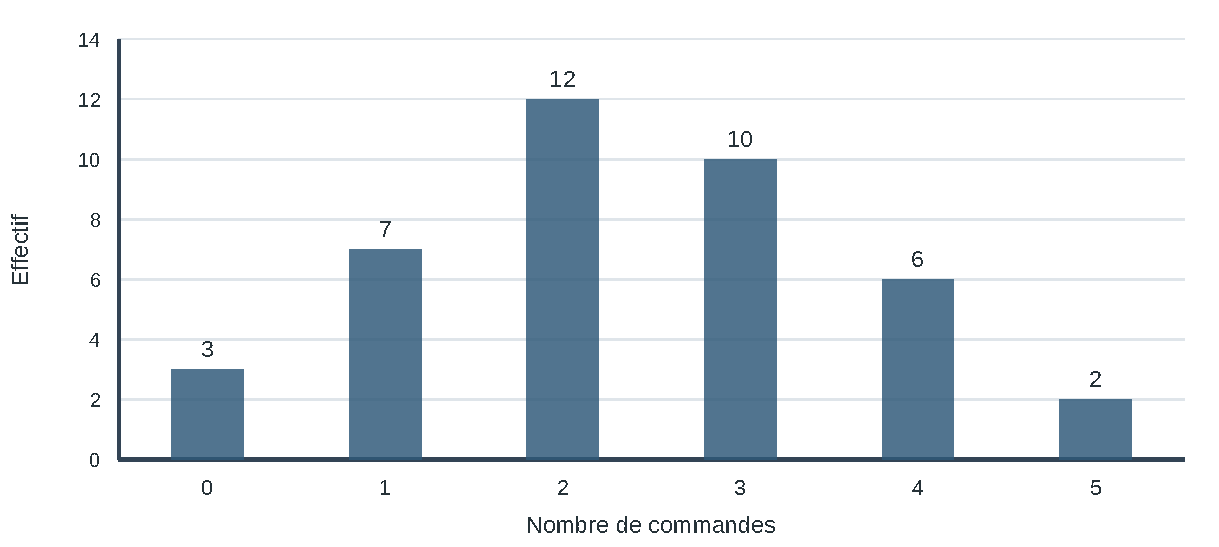
\includegraphics[width=0.85\textwidth,height=\textheight]{assets/chapter-1-solutions-fr-chart-01.pdf}

\emph{Diagramme en bâtons : nombre de commandes}

Graphiques construits à partir des effectifs : la fonction de répartition atteint 80 \% à x=3.


\includegraphics[width=0.85\textwidth,height=\textheight]{assets/chapter-1-solutions-fr-chart-02.pdf}

\emph{Nombre de commandes / Orders}


\includegraphics[width=0.85\textwidth,height=\textheight]{assets/chapter-1-solutions-fr-chart-03.pdf}

\emph{Fonction de répartition / Empirical CDF}

\hypertarget{tableau-exhaustif-des-cumuls}{%
\subsubsection{Tableau exhaustif des cumuls}\label{tableau-exhaustif-des-cumuls}}

\begin{longtable}[]{@{}lllllll@{}}
\toprule\noalign{}
x & n & f=n/40 & ECC & ECD & FCC & FCD \\
\midrule\noalign{}
\endhead
\bottomrule\noalign{}
\endlastfoot
0 & 3 & 3/40=.075 & 3 & 40 & .075 & 1.000 \\
1 & 7 & 7/40=.175 & 10 & 37 & .250 & .925 \\
2 & 12 & 12/40=.300 & 22 & 30 & .550 & .750 \\
3 & 10 & 10/40=.250 & 32 & 18 & .800 & .450 \\
4 & 6 & 6/40=.150 & 38 & 8 & .950 & .200 \\
5 & 2 & 2/40=.050 & 40 & 2 & 1.000 & .050 \\
\end{longtable}

À x=3, ECC=3+7+12+10=32 et ECD=10+6+2=18. Les fréquences cumulées croissantes mesurent P(X≤x), les décroissantes P(X≥x).

\emph{Application du cours --- 15 min}

\hypertarget{compluxe9ment-1-tableau-croisuxe9-et-pourcentages-conditionnels}{%
\subsection{Complément 1 --- Tableau croisé et pourcentages conditionnels}\label{compluxe9ment-1-tableau-croisuxe9-et-pourcentages-conditionnels}}

Parmi 120 étudiants, 50 utilisent les transports publics, dont 30 femmes. Parmi les 70 autres étudiants, 35 sont des femmes.

\begin{enumerate}
\tightlist
\item
  Construisez le tableau sexe × transport.
\item
  Calculez le taux d'utilisation des transports publics dans chaque groupe.
\item
  Indiquez si une association semble présente.
\end{enumerate}

\textbf{Indication méthodologique :}

Un pourcentage conditionnel utilise comme dénominateur le total du groupe conditionnant.

\hypertarget{corriguxe9-duxe9tailluxe9-2}{%
\subsubsection{Corrigé détaillé}\label{corriguxe9-duxe9tailluxe9-2}}

Tableau : femmes 30 « public » et 35 « autre » ; hommes 20 et 35. Totaux : 65 femmes et 55 hommes. Les taux conditionnels sont 30/65 = 46,2 \% et 20/55 = 36,4 \%.

L'écart observé vaut 9,8 points. Il décrit une association dans l'échantillon, sans démontrer une différence dans la population ni un effet causal.

\hypertarget{pruxe9paration-aux-uxe9valuations}{%
\section{Préparation aux évaluations}\label{pruxe9paration-aux-uxe9valuations}}

Résoudre des exercices de contrôle continu et de partiel en autonomie.

\emph{Préparation CC / partiel --- 40 min}

\hypertarget{exercice-3-variable-continue-et-classes-damplitudes-inuxe9gales}{%
\subsection{Exercice 3 -- Variable continue et classes d'amplitudes inégales}\label{exercice-3-variable-continue-et-classes-damplitudes-inuxe9gales}}

On observe le prix maximal, en euros, que 210 clients sont prêts à payer :

\begin{longtable}[]{@{}llllllllll@{}}
\toprule\noalign{}
Classe & {\([10,14[\)} & {\([14,18[\)} & {\([18,26[\)} & {\([26,30[\)} & {\([30,35[\)} & {\([35,40[\)} & {\([40,45[\)} & {\([45,50[\)} & {\([50,55[\)} \\
\midrule\noalign{}
\endhead
\bottomrule\noalign{}
\endlastfoot
{\(n_i\)} & 4 & 12 & 32 & 32 & 60 & 35 & 25 & 5 & 5 \\
\end{longtable}

\begin{enumerate}
\item
  Calculer, pour chaque classe, l'amplitude {\(a_i\)}, la fréquence {\(f_i\)} et la densité d'effectif {\(d_i=n_i/a_i\)}.
\item
  Construire l'histogramme correct et expliquer pourquoi la hauteur ne peut pas être directement l'effectif lorsque les amplitudes sont différentes.
\item
  Calculer les effectifs cumulés croissants (ECC) et décroissants (ECD), ainsi que les fréquences cumulées correspondantes.
\item
  Tracer les courbes cumulatives.
\item
  Déterminer le nombre et la proportion de clients prêts à payer moins de 35 euros, puis au moins 35 euros.
\end{enumerate}

\hypertarget{corriguxe9-duxe9tailluxe9-3}{%
\subsubsection{Corrigé détaillé}\label{corriguxe9-duxe9tailluxe9-3}}

\begin{longtable}[]{@{}llllllllll@{}}
\toprule\noalign{}
Classe & {\([10,14[\)} & {\([14,18[\)} & {\([18,26[\)} & {\([26,30[\)} & {\([30,35[\)} & {\([35,40[\)} & {\([40,45[\)} & {\([45,50[\)} & {\([50,55[\)} \\
\midrule\noalign{}
\endhead
\bottomrule\noalign{}
\endlastfoot
{\(n_i\)} & 4 & 12 & 32 & 32 & 60 & 35 & 25 & 5 & 5 \\
{\(a_i\)} & 4 & 4 & 8 & 4 & 5 & 5 & 5 & 5 & 5 \\
{\(f_i(\%)\)} & 1.90 & 5.71 & 15.24 & 15.24 & 28.57 & 16.67 & 11.90 & 2.38 & 2.38 \\
{\(d_i\)} & 1 & 3 & 4 & 8 & 12 & 7 & 5 & 1 & 1 \\
ECC & 4 & 16 & 48 & 80 & 140 & 175 & 200 & 205 & 210 \\
ECD & 210 & 206 & 194 & 162 & 130 & 70 & 35 & 10 & 5 \\
\end{longtable}

Par exemple : {\[f_{[18,26[}=\frac{32}{210}\approx0.1524=15.24\%,
\qquad
d_{[18,26[}=\frac{32}{8}=4.\]} Lorsque les largeurs de classes diffèrent, c'est l'aire du rectangle qui doit représenter l'effectif. On utilise donc la densité comme hauteur.

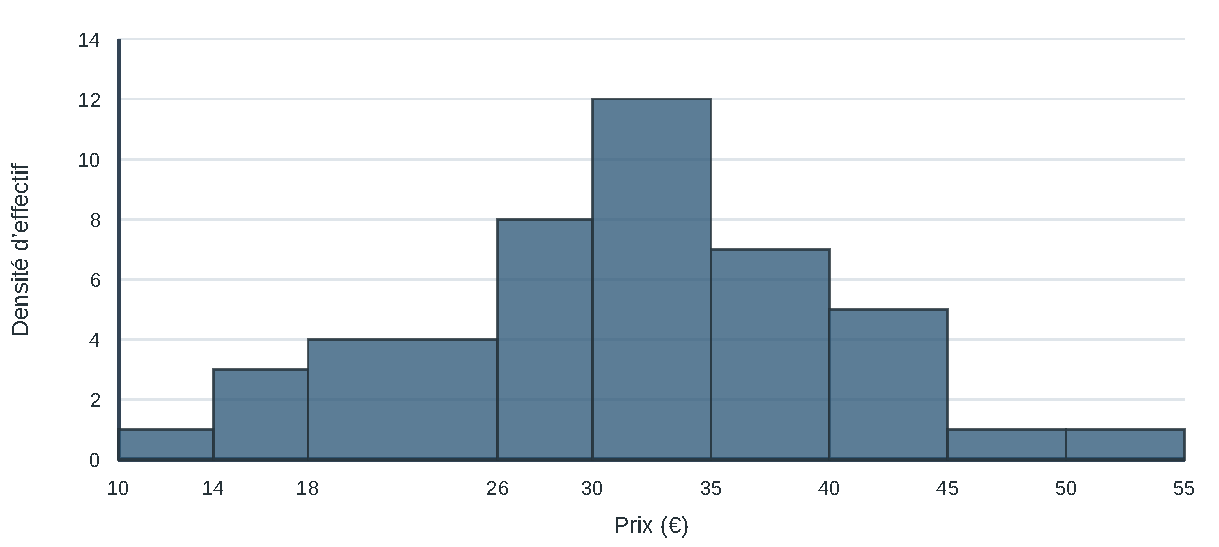
\includegraphics[width=0.85\textwidth,height=\textheight]{assets/chapter-1-solutions-fr-chart-04.pdf}

\emph{Histogramme à classes d'amplitudes inégales}

Sous 35 euros : {\[4+12+32+32+60=140,
\qquad
\frac{140}{210}=66.67\%.\]} Au moins 35 euros : {\[35+25+5+5=70,
\qquad
\frac{70}{210}=33.33\%.\]}

Tableau exhaustif : fᵢ=nᵢ/210 ; FCC=ECC/210 ; FCD=ECD/210. Les courbes cumulées utilisent les bornes des classes.

\begin{longtable}[]{@{}lllllllll@{}}
\toprule\noalign{}
Classe & aᵢ & nᵢ & fᵢ (\%) & dᵢ & ECC & ECD & FCC (\%) & FCD (\%) \\
\midrule\noalign{}
\endhead
\bottomrule\noalign{}
\endlastfoot
{[}10,14{[} & 4 & 4 & 1.90 & 1 & 4 & 210 & 1.90 & 100.00 \\
{[}14,18{[} & 4 & 12 & 5.71 & 3 & 16 & 206 & 7.62 & 98.10 \\
{[}18,26{[} & 8 & 32 & 15.24 & 4 & 48 & 194 & 22.86 & 92.38 \\
{[}26,30{[} & 4 & 32 & 15.24 & 8 & 80 & 162 & 38.10 & 77.14 \\
{[}30,35{[} & 5 & 60 & 28.57 & 12 & 140 & 130 & 66.67 & 61.90 \\
{[}35,40{[} & 5 & 35 & 16.67 & 7 & 175 & 70 & 83.33 & 33.33 \\
{[}40,45{[} & 5 & 25 & 11.90 & 5 & 200 & 35 & 95.24 & 16.67 \\
{[}45,50{[} & 5 & 5 & 2.38 & 1 & 205 & 10 & 97.62 & 4.76 \\
{[}50,55{[} & 5 & 5 & 2.38 & 1 & 210 & 5 & 100.00 & 2.38 \\
TOTAL & --- & 210 & 100 & --- & 210 & --- & 100 & --- \\
\end{longtable}


\includegraphics[width=0.85\textwidth,height=\textheight]{assets/chapter-1-solutions-fr-chart-05.pdf}

\emph{Histogramme des densités / Density histogram}


\includegraphics[width=0.85\textwidth,height=\textheight]{assets/chapter-1-solutions-fr-chart-06.pdf}

\emph{Effectifs cumulés / Cumulative counts}

\emph{Préparation CC / partiel --- 35 min}

\hypertarget{compluxe9ment-3-cas-de-pruxe9paration-au-contruxf4le-consentement-uxe0-payer}{%
\subsection{Complément 3 --- Cas de préparation au contrôle : consentement à payer}\label{compluxe9ment-3-cas-de-pruxe9paration-au-contruxf4le-consentement-uxe0-payer}}

\textbf{Étude de cas --- 12 points.} Une enseigne alimentaire interroge 200 clients sur le prix maximal qu'ils accepteraient de payer pour une boîte-repas durable.

\begin{longtable}[]{@{}lllllll@{}}
\toprule\noalign{}
Prix maximal (€) & {[}20,25{[} & {[}25,30{[} & {[}30,40{[} & {[}40,50{[} & {[}50,60{[} & {[}60,80{[} \\
\midrule\noalign{}
\endhead
\bottomrule\noalign{}
\endlastfoot
Clients & 10 & 20 & 50 & 60 & 40 & 20 \\
\end{longtable}

\begin{enumerate}
\tightlist
\item
  Identifiez la population, l'unité statistique, la variable et sa nature. \emph{(2 points)}
\item
  Calculez les amplitudes, les fréquences relatives et les densités. \emph{(3 points)}
\item
  Expliquez la construction de l'histogramme correct et identifiez la classe modale. \emph{(2 points)}
\item
  Calculez les effectifs cumulés croissants et décroissants. Donnez les coordonnées nécessaires aux deux courbes cumulées. \emph{(3 points)}
\item
  Déterminez le prix maximal qu'au moins 60 \% des clients interrogés accepteraient de payer. Expliquez le percentile utilisé. \emph{(2 points)}
\end{enumerate}

\textbf{Indication méthodologique :}

Avec des classes d'amplitudes différentes, utilisez les densités. Pour la décision de prix, traduisez « au moins 60 \% peuvent payer » en pourcentage cumulé croissant.

\hypertarget{corriguxe9-duxe9tailluxe9-4}{%
\subsubsection{Corrigé détaillé}\label{corriguxe9-duxe9tailluxe9-4}}

\hypertarget{corriguxe9-duxe9tailluxe9-et-logique-du-baruxe8me}{%
\subsubsection{Corrigé détaillé et logique du barème}\label{corriguxe9-duxe9tailluxe9-et-logique-du-baruxe8me}}

\textbf{1.} Population : les 200 clients interrogés ; unité : un client interrogé ; variable : consentement maximal à payer en euros ; nature : quantitative continue.

\begin{longtable}[]{@{}llllll@{}}
\toprule\noalign{}
Classe & Amplitude & Effectif & Fréquence & Densité & ECC \\
\midrule\noalign{}
\endhead
\bottomrule\noalign{}
\endlastfoot
{[}20,25{[} & 5 & 10 & 5 \% & 2 & 10 \\
{[}25,30{[} & 5 & 20 & 10 \% & 4 & 30 \\
{[}30,40{[} & 10 & 50 & 25 \% & 5 & 80 \\
{[}40,50{[} & 10 & 60 & 30 \% & 6 & 140 \\
{[}50,60{[} & 10 & 40 & 20 \% & 4 & 180 \\
{[}60,80{[} & 20 & 20 & 10 \% & 1 & 200 \\
\end{longtable}

\textbf{2--3.} Les amplitudes étant différentes, les hauteurs de l'histogramme sont les densités et non les effectifs bruts. La densité maximale vaut 6 : la classe modale est {[}40,50{[}.

\textbf{4.} La courbe croissante passe par (20,0), (25,10), (30,30), (40,80), (50,140), (60,180), (80,200). La courbe décroissante utilise (20,200), (25,190), (30,170), (40,120), (50,60), (60,20), (80,0).

\textbf{5.} Si au moins 60 \% doivent pouvoir payer, au plus 40 \% peuvent avoir un consentement inférieur au prix choisi. Quarante pour cent de 200 représentent 80 clients, seuil atteint à 40 €. On utilise donc le 40e percentile, et non le 60e : le prix maximal recommandé est \textbf{40 €}.

\textbf{Réflexe d'évaluation.} Énoncez la règle, présentez le calcul, puis interprétez le résultat dans le contexte de la décision.

Tableau intégral et représentations graphiques (hauteurs de l\textquotesingle histogramme = effectifs/amplitudes) :

\begin{longtable}[]{@{}lllllllll@{}}
\toprule\noalign{}
Classe / Class & nᵢ & aᵢ & fᵢ (\%) & dᵢ & ECC & ECD & FCC (\%) & FCD (\%) \\
\midrule\noalign{}
\endhead
\bottomrule\noalign{}
\endlastfoot
{[}20,25{[} & 10 & 5 & 5.00 & 2 & 10 & 200 & 5.00 & 100.00 \\
{[}25,30{[} & 20 & 5 & 10.00 & 4 & 30 & 190 & 15.00 & 95.00 \\
{[}30,40{[} & 50 & 10 & 25.00 & 5 & 80 & 170 & 40.00 & 85.00 \\
{[}40,50{[} & 60 & 10 & 30.00 & 6 & 140 & 120 & 70.00 & 60.00 \\
{[}50,60{[} & 40 & 10 & 20.00 & 4 & 180 & 60 & 90.00 & 30.00 \\
{[}60,80{[} & 20 & 20 & 10.00 & 1 & 200 & 20 & 100.00 & 10.00 \\
\end{longtable}


\includegraphics[width=0.85\textwidth,height=\textheight]{assets/chapter-1-solutions-fr-chart-07.pdf}

\emph{Consentement à payer / Willingness-to-pay histogram}


\includegraphics[width=0.85\textwidth,height=\textheight]{assets/chapter-1-solutions-fr-chart-08.pdf}

\emph{Courbes cumulatives / Cumulative counts}

Le seuil de 40 € est le 40e percentile : 80 clients sur 200 acceptent moins de 40 €, donc environ 60 \% peuvent payer au moins 40 €.

\emph{Préparation CC / partiel --- 30 min}

\hypertarget{compluxe9ment-4-synthuxe8se-type-examen-pruxe9senter-la-satisfaction-client}{%
\subsection{Complément 4 --- Synthèse type examen : présenter la satisfaction client}\label{compluxe9ment-4-synthuxe8se-type-examen-pruxe9senter-la-satisfaction-client}}

\textbf{Cas autonome --- 10 points.} Deux magasins recueillent la satisfaction sur une échelle ordonnée de 1 (très insatisfait) à 5 (très satisfait).

\begin{longtable}[]{@{}lllllll@{}}
\toprule\noalign{}
Note & 1 & 2 & 3 & 4 & 5 & Total \\
\midrule\noalign{}
\endhead
\bottomrule\noalign{}
\endlastfoot
Magasin A & 6 & 10 & 18 & 36 & 30 & 100 \\
Magasin B & 4 & 12 & 30 & 34 & 20 & 100 \\
\end{longtable}

\begin{enumerate}
\tightlist
\item
  Identifiez la variable et son échelle de mesure. \emph{(1 point)}
\item
  Choisissez et justifiez un graphique permettant de comparer les deux magasins. Décrivez précisément sa construction. \emph{(2 points)}
\item
  Calculez, pour chaque magasin, la proportion de notes 4 ou 5 et le pourcentage cumulé de notes inférieures ou égales à 2. \emph{(3 points)}
\item
  Un responsable affirme : « Le magasin A est 50 \% meilleur, car il obtient 30 notes de 5 contre 20. » Critiquez cette affirmation. \emph{(2 points)}
\item
  Rédigez une conclusion statistique en trois phrases incluant une limite de l'enquête. \emph{(2 points)}
\end{enumerate}

\textbf{Indication méthodologique :}

Conservez l'ordre des modalités, comparez les pourcentages et distinguez description et causalité.

\hypertarget{corriguxe9-duxe9tailluxe9-5}{%
\subsubsection{Corrigé détaillé}\label{corriguxe9-duxe9tailluxe9-5}}

\textbf{1.} La satisfaction est qualitative ordinale : les modalités sont ordonnées, mais les écarts entre deux notes successives ne sont pas nécessairement égaux.

\textbf{2.} Utiliser des barres groupées ou des barres empilées à 100 \%, en conservant l'ordre 1--5, avec les mêmes axes et les pourcentages. Un histogramme ne convient pas : les modalités sont ordinales et non des intervalles continus.

\textbf{3.} Magasin A : notes 4--5 = (36+30)/100 = \textbf{66 \%} ; notes au plus égales à 2 = (6+10)/100 = \textbf{16 \%}. Magasin B : notes 4--5 = (34+20)/100 = \textbf{54 \%} ; notes au plus égales à 2 = (4+12)/100 = \textbf{16 \%}.

\textbf{4.} Trente est bien supérieur de 50 \% à vingt, mais ce calcul isole une seule modalité et ne signifie pas que le magasin est « 50 \% meilleur ». Pour les notes 4--5, l'écart est de 12 points ; la méthode d'échantillonnage et l'incertitude sont inconnues, et aucune causalité n'est établie.

\textbf{5. Conclusion modèle.} « Dans les échantillons interrogés, le magasin A présente davantage de notes favorables (66 \%) que le magasin B (54 \%), tandis que les deux magasins comptent 16 \% de notes 1 ou 2. Cette différence reste descriptive et ne prouve pas à elle seule que le magasin A offre un meilleur service. Avant toute généralisation, il faut connaître la sélection des clients, les taux de réponse et la comparabilité des périodes. »

\hypertarget{approfondissement-facultatif}{%
\section{Approfondissement facultatif}\label{approfondissement-facultatif}}

Aller plus loin dans l'interprétation et les applications professionnelles.

\emph{Approfondissement --- 15 min}

\hypertarget{compluxe9ment-2-protocole-de-qualituxe9-et-de-communication}{%
\subsection{Complément 2 --- Protocole de qualité et de communication}\label{compluxe9ment-2-protocole-de-qualituxe9-et-de-communication}}

Un export CRM contient des clients dupliqués, des âges manquants codés 999, des dates incohérentes et des revenus saisis en euros ou en milliers d'euros. Proposez un protocole reproductible en six étapes avant de produire un tableau de bord.

\textbf{Indication méthodologique :}

Séparez validation, nettoyage, documentation et communication.

\hypertarget{corriguxe9-duxe9tailluxe9-6}{%
\subsubsection{Corrigé détaillé}\label{corriguxe9-duxe9tailluxe9-6}}

\begin{enumerate}
\tightlist
\item
  Conserver un fichier brut immuable et les identifiants.
\item
  Établir un dictionnaire des variables et unités.
\item
  Détecter les doublons et définir une règle de conservation.
\item
  Recoder 999 en valeur manquante et analyser la non-réponse.
\item
  Contrôler dates, plages et cohérence logique.
\item
  Uniformiser les unités monétaires, documenter les transformations et publier les contrôles.
\end{enumerate}

On ne remplace jamais silencieusement les valeurs manquantes et on ne supprime pas automatiquement les observations inhabituelles.

\end{document}
